\documentclass{standalone}
% \documentclass{article}

\usepackage{tikz}
\usetikzlibrary{arrows}
\usetikzlibrary{decorations.markings}
\usetikzlibrary{calc}
\usetikzlibrary{shapes,snakes}

\begin{document}

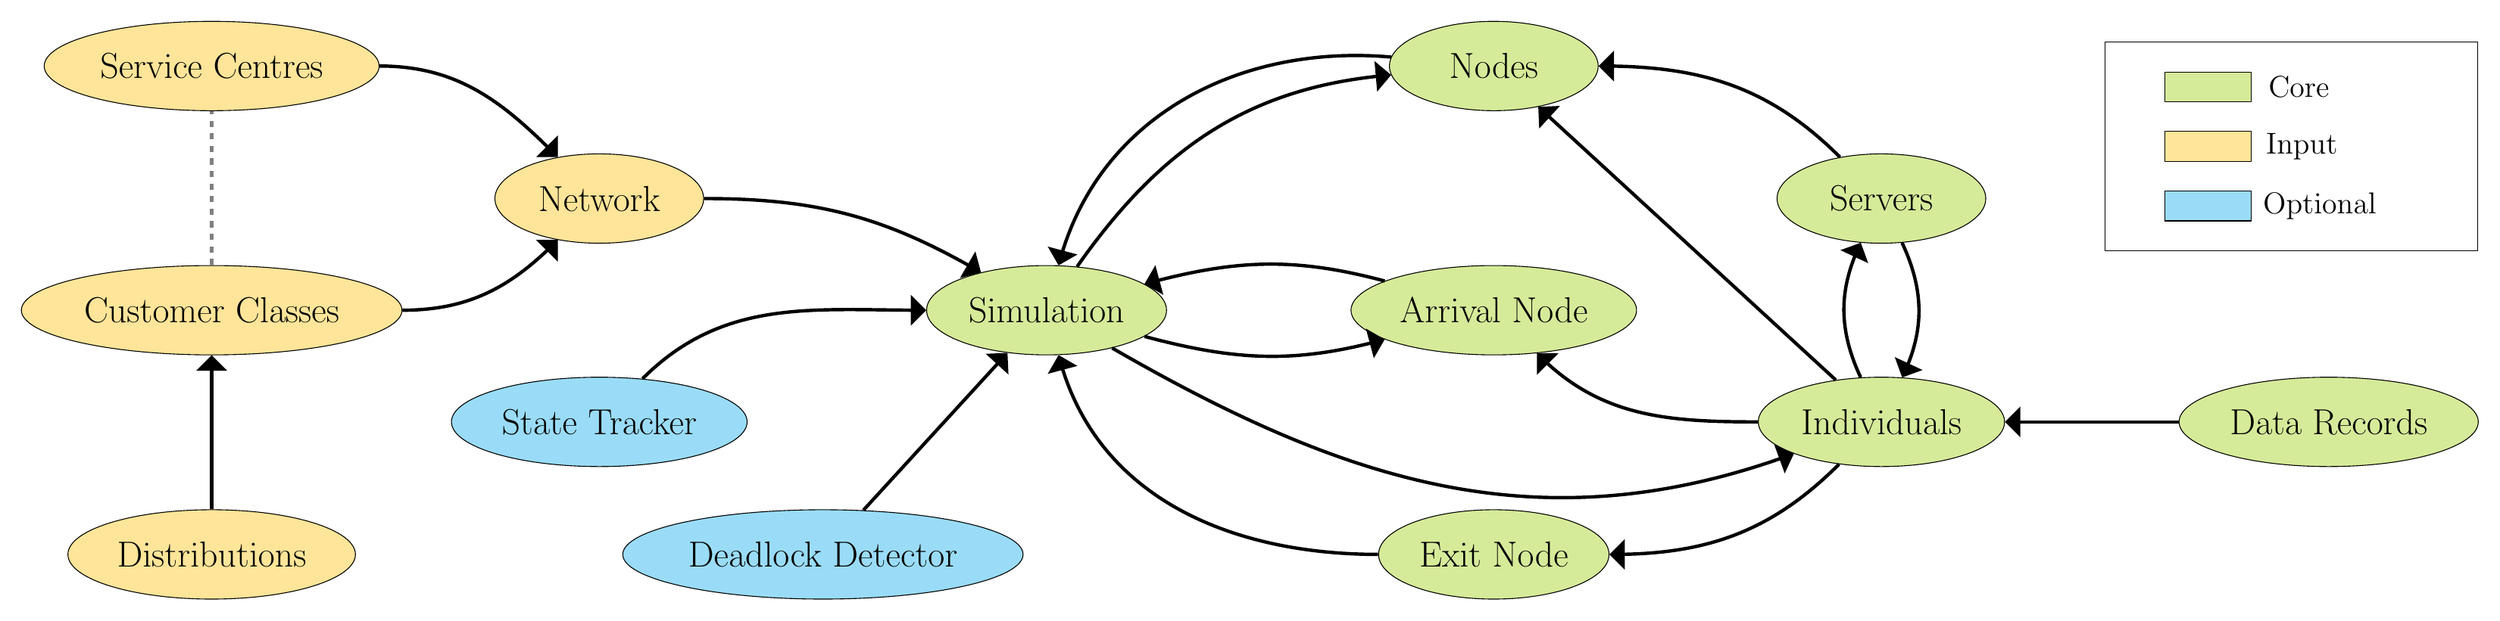
\begin{tikzpicture}

\node[align=center] (simulation) [style={minimum height=1.5cm, minimum width=3.5cm, draw=black,fill=lime!80!black,text=black,shape=ellipse,fill opacity=0.4, text opacity=1}] at (0, 0) {\LARGE Simulation};


\node[align=center] (nodes) [style={minimum height=1.5cm, minimum width=3.5cm, draw=black,fill=lime!80!black,text=black,shape=ellipse,fill opacity=0.4, text opacity=1}] at (7.5, 4.1) {\LARGE Nodes};


\node[align=center] (arrivalnode) [style={minimum height=1.5cm, minimum width=3.5cm, draw=black,fill=lime!80!black,text=black,shape=ellipse,fill opacity=0.4, text opacity=1}] at (7.5, 0) {\LARGE Arrival Node};


\node[align=center] (exitnode) [style={minimum height=1.5cm, minimum width=3.5cm, draw=black,fill=lime!80!black,text=black,shape=ellipse,fill opacity=0.4, text opacity=1}] at (7.5, -4.1) {\LARGE Exit Node};


\node[align=center] (servers) [style={minimum height=1.5cm, minimum width=3.5cm, draw=black,fill=lime!80!black,text=black,shape=ellipse,fill opacity=0.4, text opacity=1}] at (14, 1.875) {\LARGE Servers};


\node[align=center] (individuals) [style={minimum height=1.5cm, minimum width=3.5cm, draw=black,fill=lime!80!black,text=black,shape=ellipse,fill opacity=0.4, text opacity=1}] at (14, -1.875) {\LARGE Individuals};


\node[align=center] (datarecords) [style={minimum height=1.5cm, minimum width=3.5cm, draw=black,fill=lime!80!black,text=black,shape=ellipse,fill opacity=0.4, text opacity=1}] at (21.5, -1.875) {\LARGE Data Records};

\node[align=center] (network) [style={minimum height=1.5cm, minimum width=3.5cm, draw=black,fill=orange!50!yellow,text=black,shape=ellipse,fill opacity=0.4, text opacity=1}] at (-7.5, 1.875) {\LARGE Network};

\node[align=center] (servicecentre) [style={minimum height=1.5cm, minimum width=3.5cm, draw=black,fill=orange!50!yellow,text=black,shape=ellipse,fill opacity=0.4, text opacity=1}] at (-14, 4.1) {\LARGE Service Centres};

\node[align=center] (customerclass) [style={minimum height=1.5cm, minimum width=3.5cm, draw=black,fill=orange!50!yellow,text=black,shape=ellipse,fill opacity=0.4, text opacity=1}] at (-14, 0) {\LARGE Customer Classes};

\node[align=center] (distributions) [style={minimum height=1.5cm, minimum width=3.5cm, draw=black,fill=orange!50!yellow,text=black,shape=ellipse,fill opacity=0.4, text opacity=1}] at (-14, -4.1) {\LARGE Distributions};

\node[align=center] (detector) [style={minimum height=1.5cm, minimum width=3.5cm, draw=black,fill=cyan!96!blue,text=black,shape=ellipse,fill opacity=0.4, text opacity=1}] at (-3.75, -4.1) {\LARGE Deadlock Detector};

\node[align=center] (tracker) [style={minimum height=1.5cm, minimum width=3.5cm, draw=black,fill=cyan!96!blue,text=black,shape=ellipse,fill opacity=0.4, text opacity=1}] at (-7.5, -1.875) {\LARGE State Tracker};


\draw (17.75, 1) rectangle (24, 4.5);
\draw[fill=lime!80!black, fill opacity=0.4] (18.75, 3.5) rectangle (20.2, 4);
\draw[fill=orange!50!yellow, fill opacity=0.4] (18.75, 2.5) rectangle (20.2, 3);
\draw[fill=cyan!96!blue, fill opacity=0.4] (18.75, 1.5) rectangle (20.2, 2);
\node[align=left] at (21, 3.75) {\Large Core};
\node[align=left] at (21.05, 2.75) {\Large Input};
\node[align=left] at (21.35, 1.75) {\Large Optional};




\draw (datarecords) edge[ultra thick,-triangle 90] (individuals);
\draw (servers) edge[ultra thick,-triangle 90,out=-65,in=65] (individuals);
\draw (individuals) edge[ultra thick,-triangle 90,out=115,in=-115] (servers);
\draw (servers) edge[ultra thick,-triangle 90,out=135,in=0] (nodes);
\draw (individuals) edge[ultra thick,-triangle 90] (nodes);
\draw (individuals) edge[ultra thick,-triangle 90,out=180,in=-45] (arrivalnode);
\draw (individuals) edge[ultra thick,-triangle 90,out=-135,in=0] (exitnode);
\draw (nodes) edge[ultra thick,-triangle 90,out=175,in=75] (simulation);
\draw (simulation) edge[ultra thick,-triangle 90,out=55,in=-175] (nodes);
\draw (arrivalnode) edge[ultra thick,-triangle 90, out=165, in=15] (simulation);
\draw (simulation) edge[ultra thick,-triangle 90, out=-15, in=-165] (arrivalnode);
\draw (exitnode) edge[ultra thick,-triangle 90,out=180,in=-75] (simulation);
\draw (simulation) edge[ultra thick,-triangle 90,out=-30,in=-160] (individuals);

\draw (network) edge[ultra thick,-triangle 90, out=0, in=150] (simulation);
\draw (servicecentre) edge[ultra thick,-triangle 90,out=0,in=135] (network);
\draw (customerclass) edge[ultra thick,-triangle 90,out=0,in=-135] (network);
\draw (distributions) edge[ultra thick,-triangle 90,out=90,in=-90] (customerclass);

\draw (tracker) edge[ultra thick,-triangle 90,out=45,in=180] (simulation);
\draw (detector) edge[ultra thick,-triangle 90] (simulation);

\draw[draw=gray] (customerclass) edge[ultra thick, dashed] (servicecentre);

\end{tikzpicture}

\end{document}
